%%!TEX root = ./UserManual.tex
\chapter{Additional Features}
\label{chap:code}


\section{Introduction}
\label{section:AdditionalFeatureIntro}

For our bachelor thesis, we were asked to implement a couple of additional features to the original Stride project. We were requested to add two additional contact pools, being Daycare and PreSchool, and two additional data formats, being JSON and HDF5, where JSON would be used for GeoGrid's and households, and HDF5 would be just for GeoGrid's, a visualization tool which will allow the user to get a visual overview of an instance, demographic profiles, for more specific households and finally workplace size distribution, to distinguish different workplace sizes and their chance of occurring.

Each of these expansions came along with their respective implementations and tests. The following implementations were added to the system, and they are used, if not automatically, in the following manner.


%%%%%%%%%%%%%%%%%%%%%%%%%%%%%%%%%%%%%%%%%%%%%%%%%%%%%%%%%%%%%%%%
% Demographic Profile
%%%%%%%%%%%%%%%%%%%%%%%%%%%%%%%%%%%%%%%%%%%%%%%%%%%%%%%%%%%%%%%%

\section{Demographic Profile}
\label{section:demographicprofile}

\subsection{Idea}

The initial idea for this feature was that we were previously incorrectly assuming that every household is the same in the entire country. We therefore wanted to be able to read, whenever given, multiple configurations for households, so that we would be able to generate the household in a more specific manner, rather than using a general set that is the same for the entire population.

A secondary issue was that not all city types have the same household data, the major cities might have a very different ratio for young and old (which is what the differences between the household configurations are based on) than for example a smaller village might have. Since it is very difficult to determine what each city's type is, we considered the major cities versus all other cities.

\subsection{Input}
The way this data is given to stride is via the configuration file for the population. There already was a required field in the geopop\_gen section (if it exists) which was household\_file, this field will still be used, and will still be required, it will now hold the data which will be used if there is no more specific configuration at hand.

The following input fields were added, and will be used as their respective household configuration, if given. The final file is the file used to determine which cities are considered major:

\begin{description}
	\item[Antwerp]: \\ 
		antwerp\_household\_file 
	\item[Flemish Brabant]: \\
		flemish\_brabant\_household\_file
	\item[West Flanders]: \\
		west\_flanders\_household\_file
	\item[East Flanders]: \\
		east\_flanders\_household\_file
	\item[Limburg]: \\
		limburg\_household\_file
	\item[Major Cities Households]: \\
		major\_cities\_file 
	\item[Major Cities]: \\
		major\_cities
\end{description}

\subsection{New implementations for generators}
A few decisions had to be made in order to make this work. The basis was simple, we had to make a reader that read the corresponding configuration files which would store these into the memory. What was more difficult, was determining whether or not these changes should be applied to certain pools and why. The following generators are altered in the following manner.

\begin{description}
	\item[Households Generator]: 
		The $household$ $generator$ will iterate over the different regions, it will consider all locations within that region and will, for each of these locations, generate the corresponding households. It will use the given household configuration, if it was available, or the default configuration if not.
		
	\item[College Generator]:
		The $college$ $generator$ will iterate over the different regions and will generate colleges where needed, it will however not consider any specific household data, as this is irrelevant to the existence of colleges. People go to colleges all over the country, so it is more dependent on how accessible they are and how many people live in an area, rather than the possible configurations of set households in that area.
		
	\item[K12School Generator]:
		The $K12school$ $generator$ will iterate over the different specified regions and will use the possibly available data for that region. It is logical for a k12school to be dependent on the population in the surrounding environment since most of the students will generally go to a nearby k12 school. 
		
	\item[PreSchool Generator]:
		The $preschool$ $generator$ will follow the same logic as the k12school did in which it will use the specific province's/major city's household data, if available.
		
	\item[DayCare Generator]:
		The $daycare$ $generator$ will follow the same logic as the k12school did in which it will use the specific province's/major city's household data, if available.
		
	\item[Workplace Generator]:
		The $workplace$ $generator$ is a bit more difficult, in the sense that bigger workplaces will behave like the college pools did, in which they would attract people from all over the country, and other factors would become more important, while the small workplaces would behave just like K12school did, in which it would attract people from the neighboring area most of the time. We made the decision to make workplaces dependent on the household configurations of the specific areas, since almost all of the workplaces would be of a small size.
		
	\item[Primary- and Secondary Community]:
		These are not affected by household factors, and are therefore left unaltered.
\end{description}

%%%%%%%%%%%%%%%%%%%%%%%%%%%%%%%%%%%%%%%%%%%%%%%%%%%%%%%%%%%%%%%%
% Workplace Size Distribution
%%%%%%%%%%%%%%%%%%%%%%%%%%%%%%%%%%%%%%%%%%%%%%%%%%%%%%%%%%%%%%%%

\section{Workplace Size Distribtution}
\label{section:WorkplaceSizeDistribution}

\subsection{Idea}
The initial idea for this feature was based on the fact that not all workplaces are equal in size, and not all of the sizes are equally as common. In order to resolve this we added an extra input file which specifies the different sizes, along with the chance that they occur.

\subsection{Input}
This addition adds one extra, optional, input tag, $workpalce\_file$, in the geopop gen section of the populations config file which will be used to generate the workplaces.

\subsection{Workplace Generator}
Rather than creating a workplace for every 20 persons, we will now iterate for as long as we do not have sufficient space to allow all people that should work, to work. In each iteration we will generate a random size (taking in account the given chances for each size) for a new workplace pool. We will add these sizes to the geogrid configuration.

\subsection{Workplace Populator}
The Workplace populator will select a random workplace pool for each of the workers. As long as there are places left in the workplaces, these places will get priority over the other workplaces. As soon as all pools are filled to their intended size, we will randomly select pools out of all the pools within a certain range. The pools will not always get perfectly filled to their intended size, even though we intended to create an exact fit since randomness is used in the populator.

%%%%%%%%%%%%%%%%%%%%%%%%%%%%%%%%%%%%%%%%%%%%%%%%%%%%%%%%%%%%%%%%
% Data Formats
%%%%%%%%%%%%%%%%%%%%%%%%%%%%%%%%%%%%%%%%%%%%%%%%%%%%%%%%%%%%%%%%

\section{Data Formats}
\label{section:DataFormats}

\subsection{JSON: GeoGrid}
This feature offers the user to create a GeoGrid file in JSON format. These files are handled by a reader and a writer based by the concepts of "JSON for Modern C++".

If a JSON file is prefered to be used as configuration for the GeoGrid population then it is necessary to alter some attributes in the XML configuration file:\\
Change the filename of the tag \texttt{population\_file} to a file written in the JSON format.

A JSON formatted file for a GeoGrid configuration has the following attributes:
\begin{itemize}
	\item \texttt{locations} 
		: A list containing objects with:
		\begin{itemize}
			\item \texttt{id} (number)
			\item \texttt{name} (string)
			\item \texttt{province} (string)
			\item \texttt{population} (number)
			\item \texttt{coordinate} 
				\begin{itemize}
					\item \texttt{latitude} (number)
					\item \texttt{longitude} (number)
				\end{itemize}
			\item \texttt{commutes} 
				: A list with objects formatted as:
				\begin{itemize}
					\item \texttt{to} (number) : ID of a location.
					\item \texttt{proportion} (number) : Percentage of people commuting to this location.
				\end{itemize}
			\item \texttt{contactPools} 
				: List of pools per class containing the attributes:
				\begin{itemize}
					\item \texttt{class} (string defining one of the contact types)
					\item \texttt{pools} 
						: Each pool defines the persons belonging to it:
						\begin{itemize}
							\item \texttt{id} (number)
							\item \texttt{people} (list of numbers)
						\end{itemize}
				\end{itemize}
		\end{itemize}
	\item \texttt{persons}
		: A list cintaining objects with:
		\begin{itemize}
			\item \texttt{id} (number)
			\item \texttt{age} (number)
			\item \texttt{daycare} (number) : ID of pool in which this person is located.
			\item \texttt{preSchool} (number) : ID of pool in which this person is located.
			\item \texttt{k12School} (number) : ID of pool in which this person is located.
			\item \texttt{household} (number) : ID of pool in which this person is located.
			\item \texttt{workplace} (number) : ID of pool in which this person is located.
			\item \texttt{primaryCommunity} (number) : ID of pool in which this person is located.
			\item \texttt{secondaryCommunity} (number) : ID of pool in which this person is located.
			\item \texttt{college} (number) : ID of pool in which this person is located.
		\end{itemize}
\end{itemize}

\subsection{JSON: Household}
Besides reading household information in CSV format, we offered a way to provide this data in JSON format. We applied the same concept of "JSON for Modern C++" to implement a Reader that can handle such files.

If you want to use this feature and give a JSON formatted as configuration for the households then you need to change the following in the configuration XML file:
When the tag \texttt{population\_type} is in generating mode then you need to change the tag \texttt{household\_file} (within the \texttt{geopop\_gen} tag) to the name of the JSON formatted file you wish to use.

A JSON formatted file for a GeoGrid configuration has the following attributes:
\begin{itemize}
	\item \texttt{householdsName} (string)
	\item \texttt{householdsList} (list of lists of numbers) : A list with lists containing the ages within households.
\end{itemize}

\subsection{HDF5: GeoGrid}
Another supported dataformat is the HDF5 format. Hierachical DataFormat (HDF5) is a file format designed to store and organize a large amount of data. HDF5 files are defined by a .h5 extension.

If a HDF5 file is prefered to be used as configuration for the GeoGrid population then it is necessary to alter some attributes in the XML configuration file:\\
Change the filename of the tag \texttt{population\_file} to a file written in the HDF5 format.

A Geogrid formatted file written in HDF5 has the following format:

\begin{itemize}
\item \texttt{Locations} : Group
	\begin{itemize}
		\item \texttt{Location\textit{i}} : Group
			\begin{itemize}
				\item \texttt{ContactPools} : Group
					\begin{itemize}
						\item \texttt{ContactPool\textit{i}} : Dataset of unsigned ints
						\item \texttt{Commutes} : Dataset of Commute types
					\end{itemize}						
			\end{itemize}
	\end{itemize}
\item \texttt{Persons} : Dataset or Person types
\end{itemize}

\texttt{Locations}
\begin{itemize}
\item \texttt{size} : unsigned long
\end{itemize}

\texttt{Location\textit{i}}
\begin{itemize}
\item \texttt{id} : unsigned int 
\item \texttt{name} : variable length c-style string 
\item \texttt{province} : unsigned int 
\item \texttt{population} : unsigned int 
\item \texttt{longitude} : double
\item \texttt{latitude} : double
\item \texttt{size} : unsigned long
\end{itemize}

\texttt{ContactPools}
\begin{itemize}
\item \texttt{size} : unsigned long
\end{itemize}

\texttt{ContactPool\textit{i}}
\begin{itemize}
\item \texttt{id} : unsigned int 
\item \texttt{size} : unsigned long 
\item \texttt{type} : variable length c-style string
\end{itemize}

\texttt{Commutes}
\begin{itemize}
\item \texttt{size} : unsigned int
\end{itemize}

\texttt{Persons}
\begin{itemize}
\item \texttt{size} : unsigned int
\end{itemize}

%%%%%%%%%%%%%%%%%%%%%%%%%%%%%%%%%%%%%%%%%%%%%%%%%%%%%%%%%%%%%%%%
% Daycares and PreSchools
%%%%%%%%%%%%%%%%%%%%%%%%%%%%%%%%%%%%%%%%%%%%%%%%%%%%%%%%%%%%%%%%
\section{Daycares and PreSchools}
\label{section:Daycares and PreSchools}
The current implementation in stride generates contact pools for different ContactTypes and their associated AgeBrackets. There are two added ContactTypes for 0-3 years old and 3-6 years old, Daycare and Preschool. They have fixed participation rates that can't be altered via config. The participation rate for Daycare is 0.45 and the participation rate for Preschool is 0.99.

%%%%%%%%%%%%%%%%%%%%%%%%%%%%%%%%%%%%%%%%%%%%%%%%%%%%%%%%%%%%%%%%
% Data Visualization
%%%%%%%%%%%%%%%%%%%%%%%%%%%%%%%%%%%%%%%%%%%%%%%%%%%%%%%%%%%%%%%%

\section{Epidemiological output}
As input for the GUI, an epidemiological output was proposed. This \textbf{epi\_output} contains for every saved timestep the epidemiological situation. For every location the percentage of people per \textit{HealthStatus} per \textit{AgeBracket} is saved. To write this file during the simulation an extra viewer was created, the \textit{EpiViewer}. It will write the epi-output to the desired file if this was desired.\\
To create an epi-output file for a simulation add:
\begin{equation}
\begin{split}
<output\_epi>&	\\
			&<format>json</format>\\
			&<step\_size>n</step\_size>\\
</output\_epi>&
\end{split}
\end{equation}

to the config.xml file. This will make sure an epi-output file is created in JSON format with step\_size n. This n will determine how many days are skipped while writing the file. n has to be larger than 1 or no output will be generated. Make sure that locations are created (by adding geopopgen with a cities file for example) else the output will be empty. 

\subsection{Formats}
Three formats can be selected: JSON, HDF5 and protobuf. Every time the information about the locations is saved. The coordinates, name and id are saved. Then for every time the situation has to be saved, the percentage of people compared to the total population of the location is saved per AgeBracket and per HealthStatus. Below are the formats:
\subsubsection{Json}
The JSON format contains two JSON objects: the \texttt{history} and the \texttt{locations}.
\\\\
\texttt{history object:} : a list containing the following object:
\begin{itemize}
\item \texttt{timestep} : unsigned int
\item \texttt{locations} : a list containing location objects
\begin{itemize}
\item \texttt{id} : unsigned int
\item \texttt{agebrackets}
\begin{itemize}
\item \texttt{immune} 		: double
\item \texttt{susceptible} 	: double
\item \texttt{infectious} 	: double
\item \texttt{symptomatic} 	: double
\item \texttt{infectiousAndSymptomatic} 	: double
\item \texttt{recovered} 	: double
\end{itemize}
\end{itemize}
\end{itemize}

\texttt{locations object} : a list containing the following object:
\begin{itemize}
\item \texttt{coordinates}
\begin{itemize}
\item \texttt{lat} : double
\item \texttt{long} : double
\end{itemize}
\item \texttt{id} : unsigned int
\item \texttt{name} : string
\item \texttt{population} : unsigned int
\end{itemize}

\subsubsection{Protobuf}
\begin{itemize}
\item \texttt{Location} : repeated object
\begin{itemize}
\item \texttt{Coordinates} : object
\begin{itemize}
\item \texttt{latitude} : double
\item \texttt{longitude} : double
\end{itemize}
\item \texttt{id} : int32
\item \texttt{name} : string
\item \texttt{population} : int32
\end{itemize}
\end{itemize}
\begin{itemize}

\item \texttt{history} : a list containing the following object:
\begin{itemize}
\item{timestep} : int32
\item \texttt{PoolsForLocation} : repeated object
\begin{itemize}
\item \texttt{id} : int32
\item \texttt{AgeBrackt} : for every defined bracket
\begin{itemize}
\item \texttt{DayCar}	 : double (repeated)
\item \texttt{PreSchool} : double (repeated)
\item \texttt{K12School} : double (repeated)
\item \texttt{College}	 : double (repeated)
\item \texttt{Workplace} : double (repeated)
\item \texttt{Retired}	 : double (repeated)
\end{itemize}
\end{itemize}
\end{itemize}
\end{itemize}

\subsection{HDF5}
\texttt{Locations} : dataset
\begin{itemize}
\item \texttt{location}
\begin{itemize}
\item \texttt{id} : uint32
\item \texttt{population} : uint32
\item \texttt{name} : string
\item \texttt{longitude} : float64
\item \texttt{latitude} : float64
\end{itemize}
\end{itemize}

\texttt{steps} : group
\begin{itemize}
\item \texttt{locations} : group
\begin{itemize}
\item \texttt{id} : scalar
\item \texttt{AgeBrackets} : group
\begin{itemize}
\item \texttt{College} : float64 (7 times)
\item \texttt{Daycare} : float64 (7 times)
\item \texttt{K12School} : float64 (7 times)
\item \texttt{PreSchool} : float64 (7 times)
\item \texttt{Retired} : float64 (7 times)
\item \texttt{Workplace} : float64 (7 times)
\end{itemize}
\end{itemize}
\end{itemize}

\section{Data Visualization}
You can see the GUI on figure \ref{gui_location}. On the map itself, all locations have been marked with a sphere. The size of the sphere indicates the size of the population. The colour of the sphere indicates a larger percentage of people with the chosen attributes are present in the location of the sphere. \\
The attributes are the agebrackets and health statuses. You can select any combination of them in the top bar. At figure 5.1 people in college who are immune are selected. If you click on a location, that location will be selected. A smaller sphere is present in the center of any sphere so if spheres overlap you can still select the location.\\ Information about the location will be given in the sidebar on the right. The name and total selected population are given. In Antwerp there are 4091 people attending college, 10,57\% of those students are immune to the disease. Any combination of agebrackets and health statuses can be selected. If you hover the agebrackets or health statuses the full name of the button will be shown. \\
If you wish to select more locations, \textbf{Box} or \textbf{Radius} can be used. Simply click on the one you need and click on the map and drag until you have everything you need.\\
To select a different day, \textbf{Previous Day} or \textbf{Next Day} can be used to change the date.\\
To launch the GUI go to the installed location \textit{bin/gui} and use the command line \textit{./gui [filename]}. 

\begin{figure}[h]
\centering
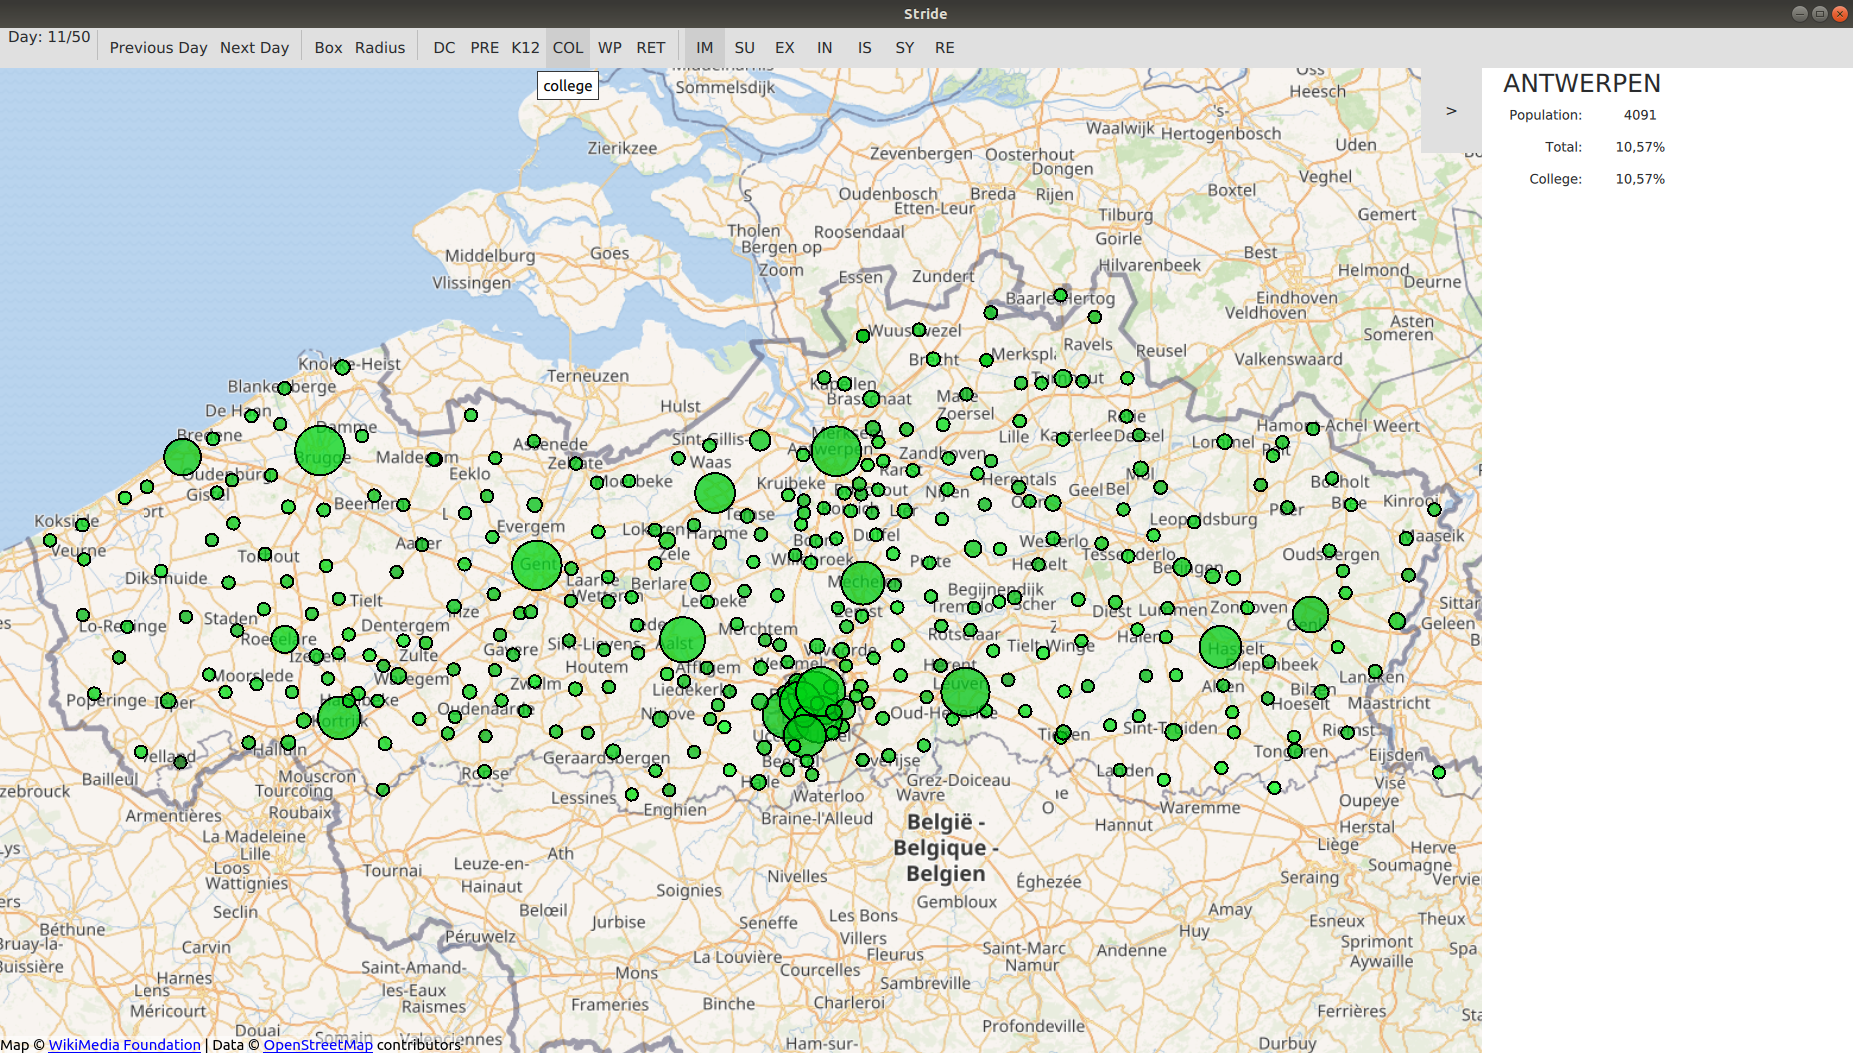
\includegraphics[width=\textwidth]{locSelect.png}
\caption{Select a location on the GUI.}
\label{gui_location}
\end{figure}




 